\chapter{Instance statistics}
\label{app:instance_stats}

\FloatBarrier
\section{Descriptives on the number of reviewed instances}

\begin{longtable}[c]{@{}lrrrrrrrrrr@{}}
    \caption{Flashcard condition}
    \endfirsthead
    \endhead
\toprule\addlinespace
& sample & min & max & mean & variance & skew & kurtosis & normal-t &
normal-p & $\alpha$
\\\addlinespace
\midrule
\textbf{abs} & 12 & 46 & 93 & 72.83 & 344.33 & -0.34 & -1.43 & 3.332 &
0.1890 & 0.9790
\\\addlinespace
\textbf{rel} & 12 & 0.49 & 1 & 0.78 & 0.04 & -0.34 & -1.43 & 3.332 & 0.1890
& 0.9790
\\\addlinespace
\bottomrule
    \label{tab:instance_fc}
\end{longtable}

\begin{figure}
    \centering
    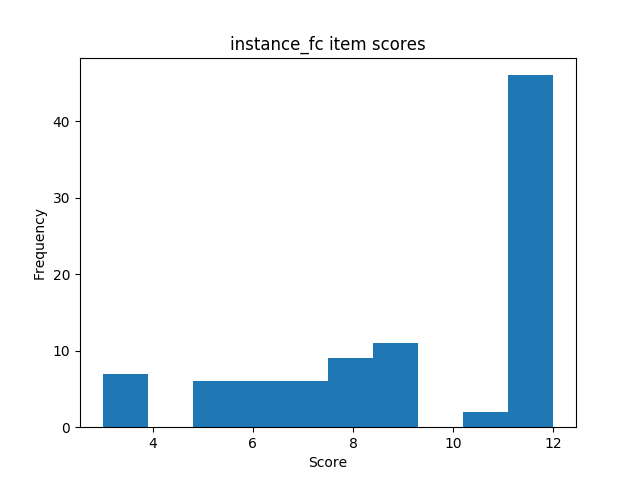
\includegraphics[width=.7\textwidth]{img/instance_fc_diff.png}
    \caption{A histogram depicting the number of reviewed instances per item given by flashcard users}
    \label{fig:instance_fc_diff}
\end{figure}
\begin{figure}
    \centering
    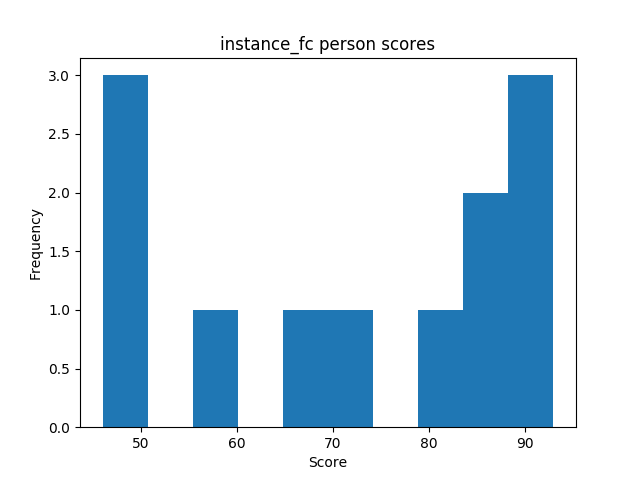
\includegraphics[width=.7\textwidth]{img/instance_fc_abil.png}
    \caption{A histogram depicting the number of reviewed instances per flashcard user}
    \label{fig:instance_fc_abil}
\end{figure}

\begin{longtable}[c]{@{}lrrrrrrrrrr@{}}
    \caption{Flashmap condition}
    \endfirsthead
    \endhead
\toprule\addlinespace
& sample & min & max & mean & variance & skew & kurtosis & normal-t &
normal-p & $\alpha$
\\\addlinespace
\midrule
\textbf{abs} & 11 & 54 & 199 & 131.45 & 2363.47 & 0.07 & -1.18 & 0.961 &
0.6186 & 0.9924
\\\addlinespace
\textbf{rel} & 11 & 0.27 & 1 & 0.66 & 0.06 & 0.07 & -1.18 & 0.961 & 0.6186
& 0.9924
\\\addlinespace
\bottomrule
    \label{tab:instance_fm}
\end{longtable}

\begin{figure}
    \centering
    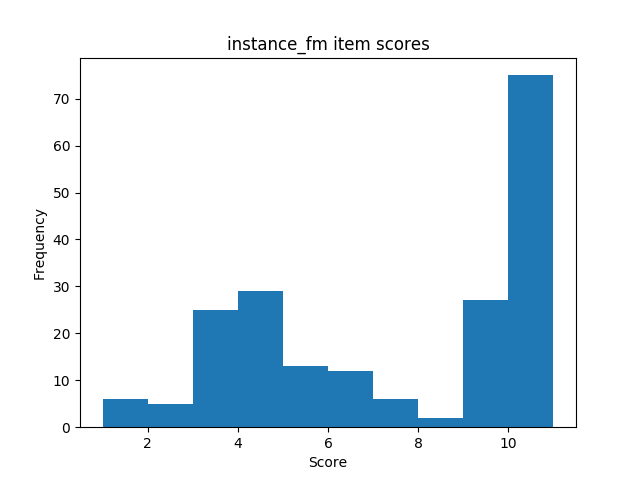
\includegraphics[width=.7\textwidth]{img/instance_fm_diff.png}
    \caption{A histogram depicting the number of reviewed instances per item given by flashmap users}
    \label{fig:instance_fm_diff}
\end{figure}
\begin{figure}
    \centering
    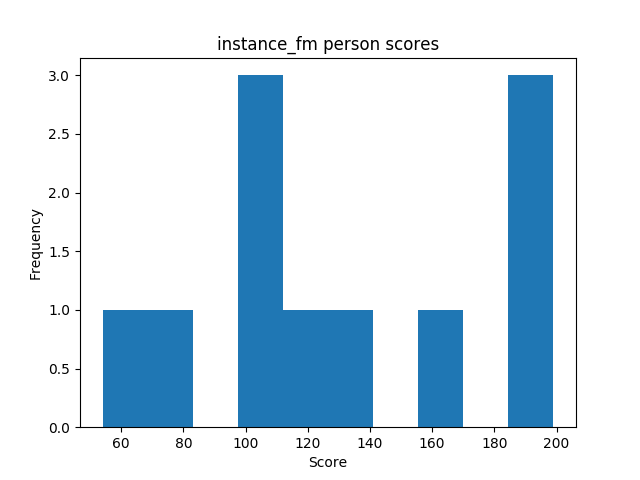
\includegraphics[width=.7\textwidth]{img/instance_fm_abil.png}
    \caption{A histogram depicting the number of reviewed instances per flashmap user}
    \label{fig:instance_fm_abil}
\end{figure}

\begin{longtable}[c]{@{}lrrrrrrrrrr@{}}
    \caption{Combined conditions}
    \endfirsthead
    \endhead
\toprule\addlinespace
& sample & min & max & mean & variance & skew & kurtosis & normal-t &
normal-p & $\alpha$
\\\addlinespace
\midrule
\textbf{rel} & 23 & 0.27 & 1 & 0.70 & 0.04 & -0.00 & -0.86 & 0.817 & 0.6647
& 0.9896
\\\addlinespace
\bottomrule
    \label{tab:instance_gen}
\end{longtable}

\section{Comparisons of reviewed instances}

\begin{longtable}[c]{@{}lrrrr@{}}
\toprule\addlinespace
& \textbf{Mann-Whitney-U k} & \textbf{Mann-Whitney-U p} &
\textbf{Welch's t-test k} & \textbf{Welch's t-test p}
\\\addlinespace
\midrule\endhead
\textbf{abs} & -3.886 & 0.0009 & -3.756 & 0.0025
\\\addlinespace
\textbf{rel} & 1.362 & 0.1875 & 1.350 & 0.1924
\\\addlinespace
\bottomrule
\end{longtable}

\begin{figure}
    \centering
    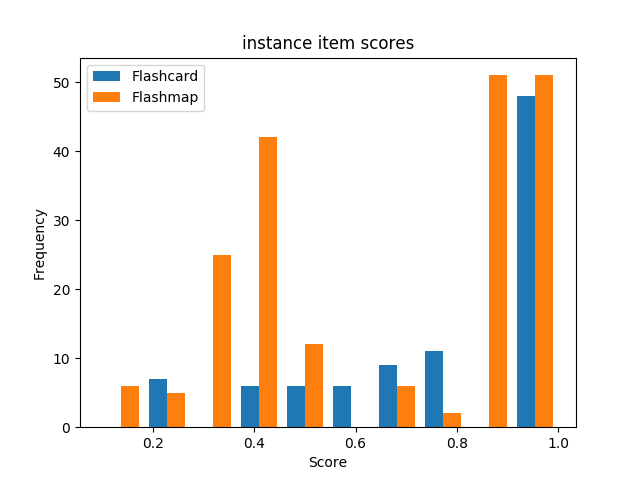
\includegraphics[width=.7\textwidth]{img/instance_diff.png}
    \caption{A comparison of figure~\protect\ref{fig:instance_fc_diff} and~\protect\ref{fig:instance_fm_diff}}
    \label{fig:instance_diff}
\end{figure}
\begin{figure}
    \centering
    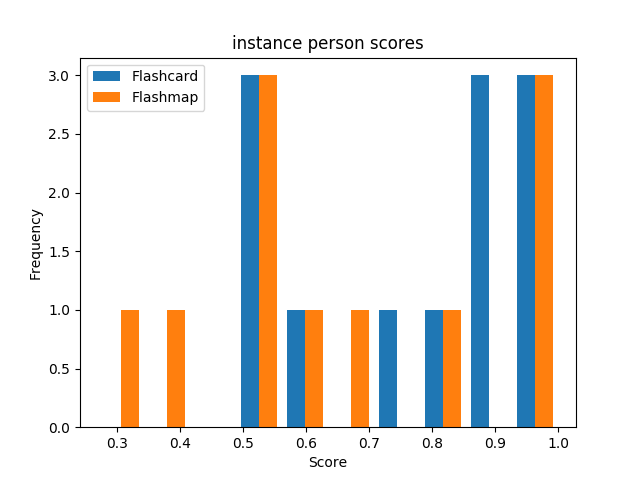
\includegraphics[width=.7\textwidth]{img/instance_abil.png}
    \caption{A comparison of figure~\protect\ref{fig:instance_fc_abil} and~\protect\ref{fig:instance_fm_abil}}
    \label{fig:instance_abil}
\end{figure}

\FloatBarrier
\section{Descriptives of the number of responses}

\begin{longtable}[c]{@{}lrrrrrrrrrr@{}}
\caption{Flashcard condition}
\endfirsthead
\endhead
\toprule\addlinespace
& N & min & max & mean & variance & skew & kurt & norm-t &
norm-p & $\alpha$
\\\addlinespace
\midrule
\textbf{abs} & 12 & 298 & 1268 & 561.33 & 70295.70 & 1.69 & 2.26 &
13.701 & 0.0011 & 0.9378
\\\addlinespace
\textbf{rel} & 12 & 3 & 13 & 6.04 & 8.13 & 1.69 & 2.26 & 13.701 & 0.0011
& 0.9378
\\\addlinespace
\textbf{mean} & 12 & 5 & 14 & 7.61 & 5.84 & 2.33 & 4.62 & 23.813 &
0.0000 & 0.9378
\\\addlinespace
\bottomrule
    \label{tab:responses_fc}
\end{longtable}

\begin{figure}
    \centering
    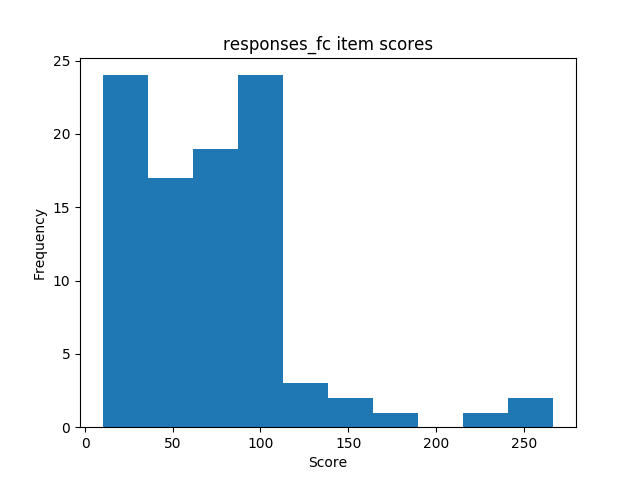
\includegraphics[width=.7\textwidth]{img/responses_fc_diff.png}
    \caption{A histogram depicting the number of responses per item given by flashcard users}
    \label{fig:responses_fc_diff}
\end{figure}
\begin{figure}
    \centering
    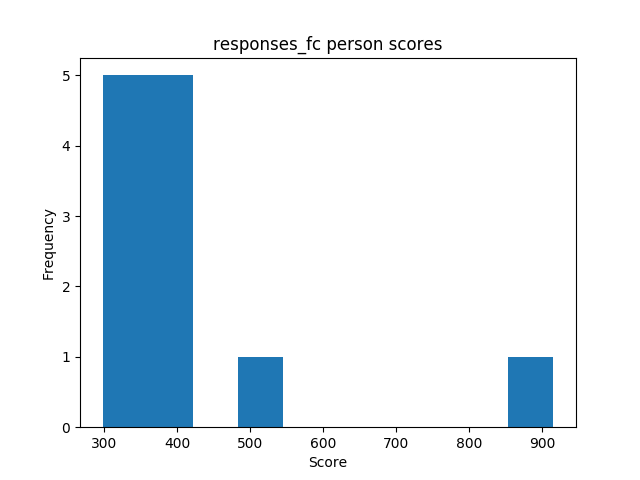
\includegraphics[width=.7\textwidth]{img/responses_fc_abil.png}
    \caption{A histogram depicting the number of responses per flashcard user}
    \label{fig:responses_fc_abil}
\end{figure}

\begin{longtable}[c]{@{}lrrrrrrrrrr@{}}
\caption{Flashmap condition}
\endfirsthead
\toprule\addlinespace
& N & min & max & mean & variance & skew & kurt & norm-t &
norm-p & $\alpha$
\\\addlinespace
\midrule
\textbf{abs} & 11 & 344 & 1555 & 729.73 & 126333.42 & 1.13 & 0.55 &
5.693 & 0.0581 & 0.9832
\\\addlinespace
\textbf{rel} & 11 & 1 & 7 & 3.67 & 3.19 & 1.13 & 0.55 & 5.693 & 0.0581 &
0.9832
\\\addlinespace
\textbf{mean} & 11 & 3 & 7 & 5.61 & 1.75 & 0.03 & -0.80 & 0.063 & 0.9690
& 0.9832
\\\addlinespace
\bottomrule
    \label{tab:responses_fm}
\end{longtable}

\begin{figure}
    \centering
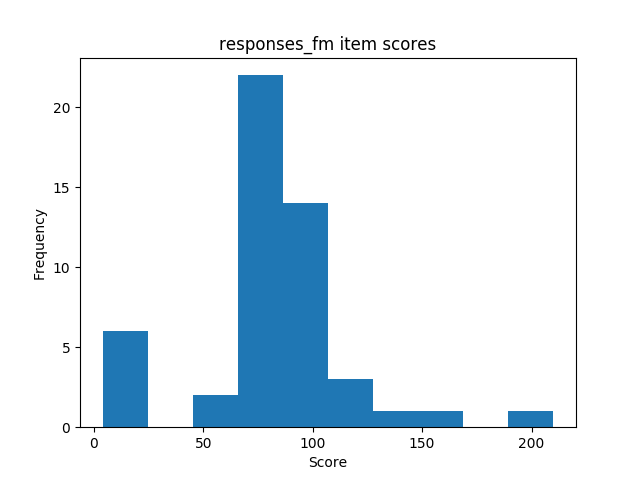
\includegraphics[width=.7\textwidth]{img/responses_fm_diff.png}
    \caption{A histogram depicting the number of responses per item given by flashmap users}
    \label{fig:responses_fm_diff}
\end{figure}
\begin{figure}
    \centering
    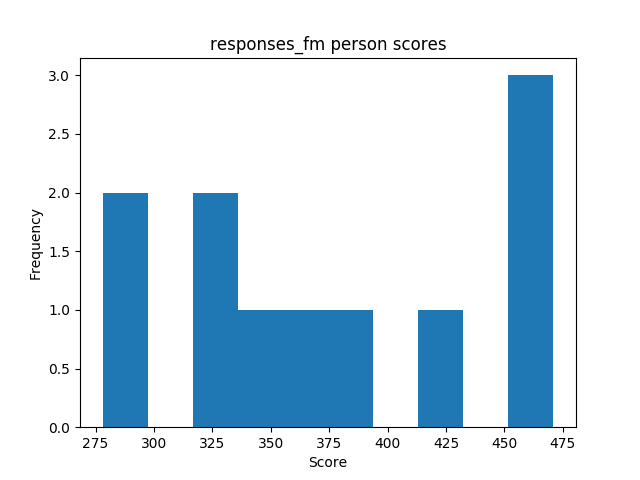
\includegraphics[width=.7\textwidth]{img/responses_fm_abil.png}
    \caption{A histogram depicting the number of responses per flashmap user}
    \label{fig:responses_fm_abil}
\end{figure}

\begin{longtable}[c]{@{}lrrrrrrrrrr@{}}
\caption{Combined conditions}
\endfirsthead
\toprule\addlinespace
& N & min & max & mean & variance & skew & kurt & norm-t &
norm-p & $\alpha$
\\\addlinespace
\midrule
\textbf{abs} & 23 & 298 & 1555 & 641.87 & 99969.48 & 1.41 & 1.42 &
11.547 & 0.0031 & 0.9579
\\\addlinespace
\textbf{mean} & 23 & 3 & 14 & 6.65 & 4.72 & 2.17 & 6.57 & 28.261 &
0.0000 & 0.9572
\\\addlinespace
\bottomrule
    \label{tab:responses_gen}
\end{longtable}

\begin{figure}
    \centering
    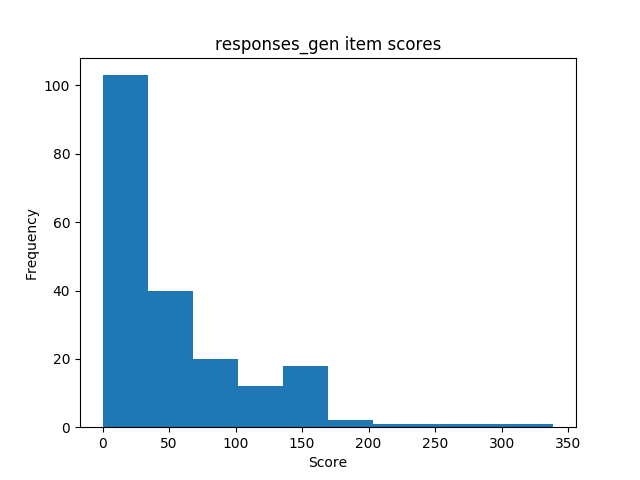
\includegraphics[width=.7\textwidth]{img/responses_gen_diff.png}
    \caption{A histogram depicting the number of responses per item}
    \label{fig:responses_gen_diff}
\end{figure}
\begin{figure}
    \centering
    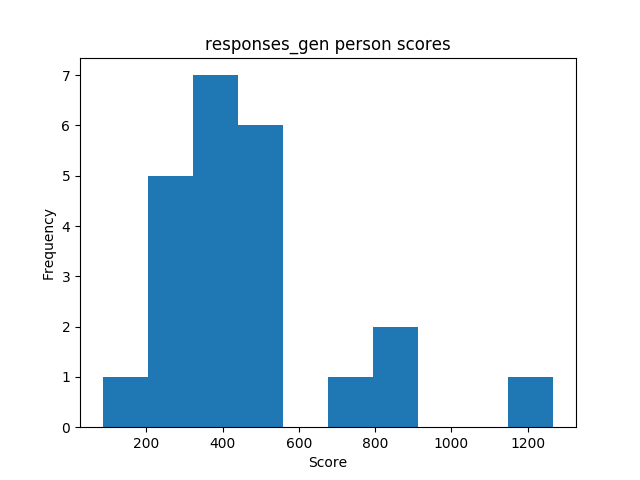
\includegraphics[width=.7\textwidth]{img/responses_gen_abil.png}
    \caption{A histogram depicting the number of responses per user}
    \label{fig:responses_gen_abil}
\end{figure}

\section{Comparisons of the number of responses}

\begin{longtable}[c]{@{}lrrrr@{}}
\toprule\addlinespace
& \textbf{MW k} & \textbf{MW p} &
\textbf{t-test k} & \textbf{t-test p}
\\\addlinespace
\midrule
\textbf{abs} & -1.295 & 0.2092 & -1.279 & 0.2169
\\\addlinespace
\textbf{rel} & 2.361 & 0.0280 & 2.409 & 0.0265
\\\addlinespace
\textbf{mean} & 2.429 & 0.0242 & 2.489 & 0.0233
\\\addlinespace
\bottomrule
    \label{tab:responses_comp}
\end{longtable}

\begin{figure}
    \centering
    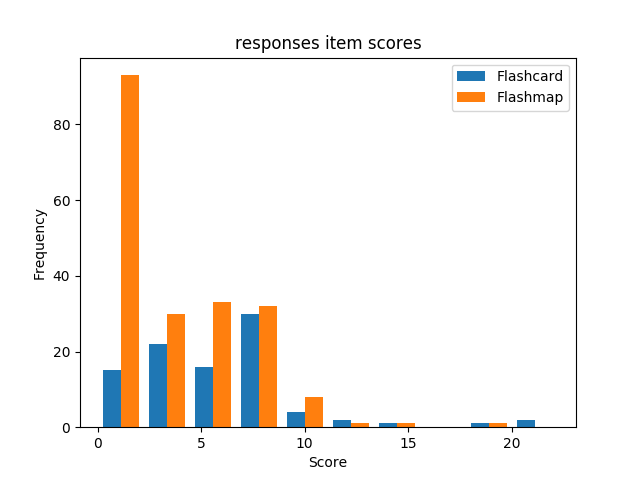
\includegraphics[width=.7\textwidth]{img/responses_diff.png}
    \caption{A comparison of figure~\protect\ref{fig:responses_fc_diff} and~\protect\ref{fig:responses_fm_diff}}
    \label{fig:responses_diff}
\end{figure}
\begin{figure}
    \centering
    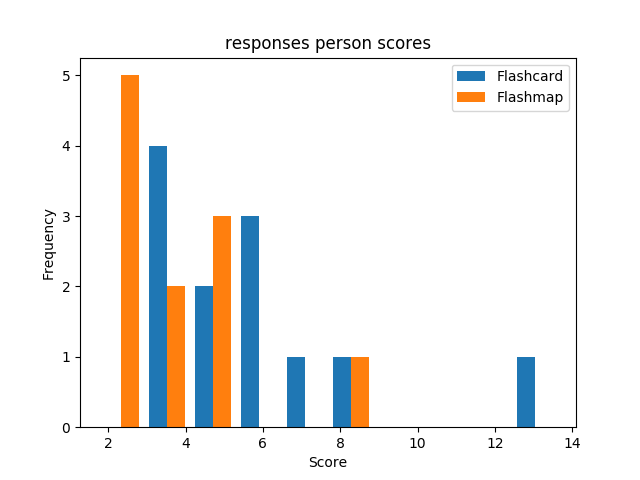
\includegraphics[width=.7\textwidth]{img/responses_abil.png}
    \caption{A comparison of figure~\protect\ref{fig:responses_fc_abil} and~\protect\ref{fig:responses_fm_abil}}
    \label{fig:responses_abil}
\end{figure}

\FloatBarrier
\section{Descriptives of the exponents of instances}

\begin{longtable}[c]{@{}lrrrrrrrrrr@{}}
    \caption{Flashcard condition}
    \endfirsthead
\toprule\addlinespace
& sample & min & max & mean & variance & skew & kurtosis & normal-t &
normal-p & $\alpha$
\\\addlinespace
\midrule
\textbf{abs} & 12 & 218 & 966 & 495.42 & 41792.81 & 0.86 & 0.42 & 3.894
& 0.1427 & 0.8933
\\\addlinespace
\textbf{rel} & 12 & 2 & 10 & 5.33 & 4.83 & 0.86 & 0.42 & 3.894 & 0.1427
& 0.8933
\\\addlinespace
\textbf{mean} & 12 & 4 & 11 & 6.67 & 2.66 & 1.83 & 3.42 & 17.448 &
0.0002 & 0.8933
\\\addlinespace
\bottomrule
    \label{tab:exponent_fc}
\end{longtable}

\begin{figure}
    \centering
    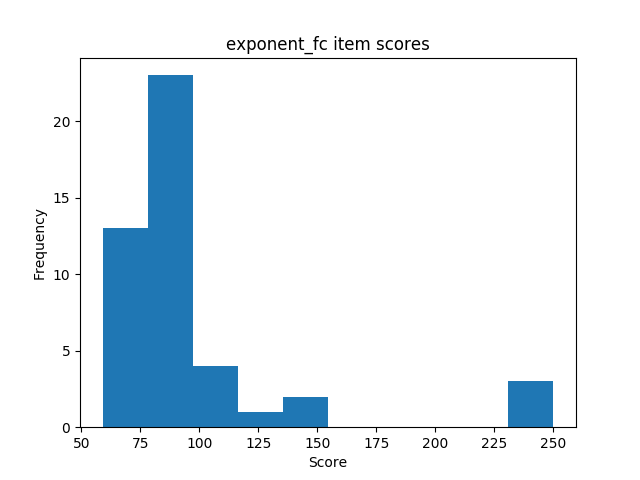
\includegraphics[width=.7\textwidth]{img/exponent_fc_diff.png}
    \caption{A histogram depicting the exponents per item of the flashcard users}
    \label{fig:exponent_fc_diff}
\end{figure}
\begin{figure}
    \centering
    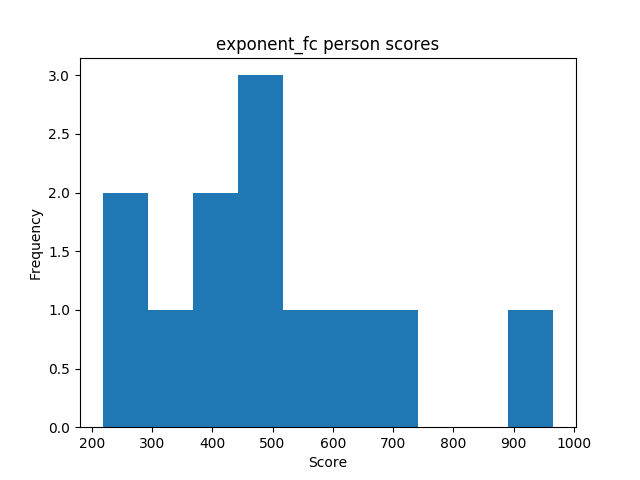
\includegraphics[width=.7\textwidth]{img/exponent_fc_abil.png}
    \caption{A histogram depicting the exponents per flashcard user}
    \label{fig:exponent_fc_abil}
\end{figure}

\begin{longtable}[c]{@{}lrrrrrrrrrr@{}}
    \caption{Flashmap condition}
    \endfirsthead
\toprule\addlinespace
& sample & min & max & mean & variance & skew & kurtosis & normal-t &
normal-p & $\alpha$
\\\addlinespace
\midrule
\textbf{abs} & 11 & 330 & 1523 & 842.27 & 132229.22 & 0.67 & -0.65 &
1.467 & 0.4803 & 0.9800
\\\addlinespace
\textbf{rel} & 11 & 1 & 7 & 4.21 & 3.31 & 0.67 & -0.65 & 1.467 & 0.4803
& 0.9800
\\\addlinespace
\textbf{mean} & 11 & 5 & 8 & 6.38 & 1.01 & 1.14 & 0.11 & 4.835 & 0.0891
& 0.9800
\\\addlinespace
\bottomrule
    \label{tab:exponent_fm}
\end{longtable}

\begin{figure}
    \centering
    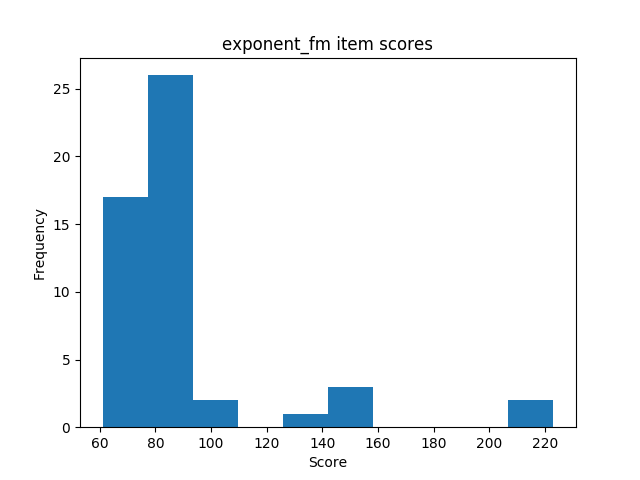
\includegraphics[width=.7\textwidth]{img/exponent_fm_diff.png}
    \caption{A histogram depicting the exponents per item of the flashmap users}
    \label{fig:exponent_fm_diff}
\end{figure}
\begin{figure}
    \centering
    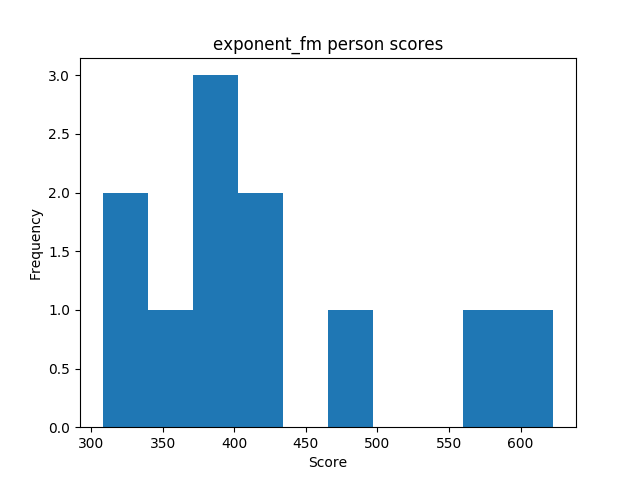
\includegraphics[width=.7\textwidth]{img/exponent_fm_abil.png}
    \caption{A histogram depicting the exponents per flashmap user}
    \label{fig:exponent_fm_abil}
\end{figure}

\begin{longtable}[c]{@{}lrrrrrrrrrr@{}}
    \caption{Combined conditions}
    \endfirsthead
\toprule\addlinespace
& sample & min & max & mean & variance & skew & kurtosis & normal-t &
normal-p & $\alpha$
\\\addlinespace
\midrule
\textbf{abs} & 23 & 218 & 1523 & 661.30 & 112385.58 & 1.09 & 0.62 &
6.912 & 0.0316 & 0.9632
\\\addlinespace
\textbf{mean} & 23 & 4 & 11 & 6.53 & 1.81 & 1.95 & 4.68 & 23.191 &
0.0000 & 0.9632
\\\addlinespace
\bottomrule
    \label{tab:exponent_gen}
\end{longtable}

\begin{figure}
    \centering
    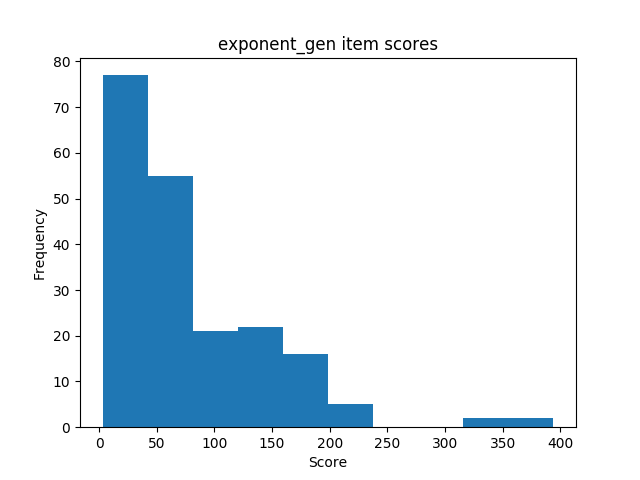
\includegraphics[width=.7\textwidth]{img/exponent_gen_diff.png}
    \caption{A histogram depicting the exponents per item}
    \label{fig:exponent_gen_diff}
\end{figure}
\begin{figure}
    \centering
    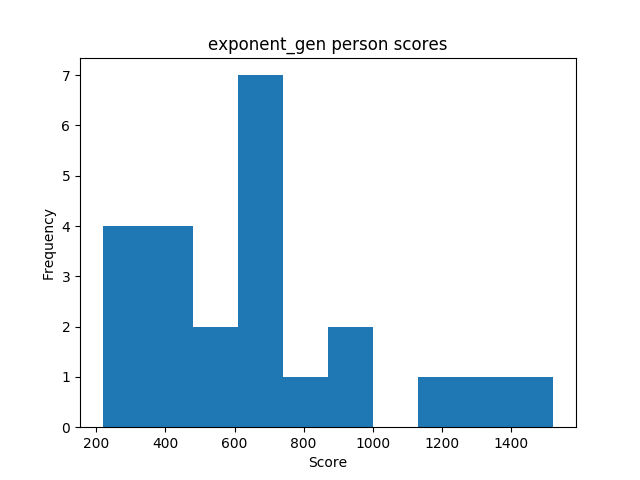
\includegraphics[width=.7\textwidth]{img/exponent_gen_abil.png}
    \caption{A histogram depicting the exponents per user}
    \label{fig:exponent_gen_abil}
\end{figure}

\section{Comparisons of the exponents}

\begin{longtable}[c]{@{}lrrrr@{}}
\toprule\addlinespace
& \textbf{Mann-Whitney-U k} & \textbf{Mann-Whitney-U p} &
\textbf{Welch's t-test k} & \textbf{Welch's t-test p}
\\\addlinespace
\midrule\endhead
\textbf{abs} & -2.853 & 0.0095 & -2.786 & 0.0136
\\\addlinespace
\textbf{rel} & 1.319 & 0.2013 & 1.330 & 0.1978
\\\addlinespace
\textbf{mean} & 0.497 & 0.6246 & 0.507 & 0.6182
\\\addlinespace
\bottomrule
    \label{tab:exponent_comp}
\end{longtable}

\begin{figure}
    \centering
    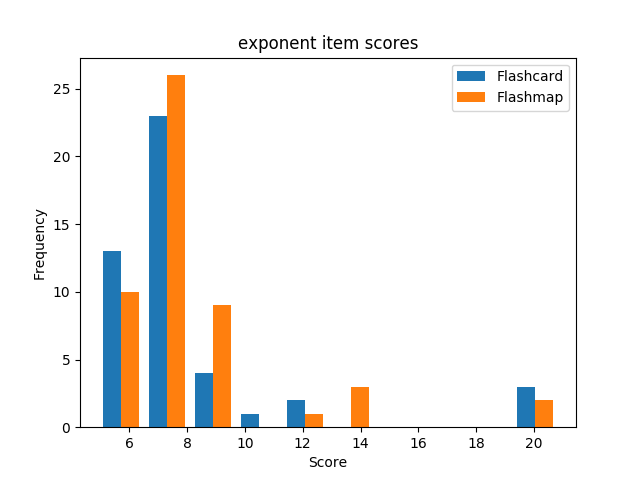
\includegraphics[width=.7\textwidth]{img/exponent_diff.png}
    \caption{A comparison of figure~\protect\ref{fig:exponent_fc_diff} and~\protect\ref{fig:exponent_fm_diff}}
    \label{fig:exponent_diff}
\end{figure}
\begin{figure}
    \centering
    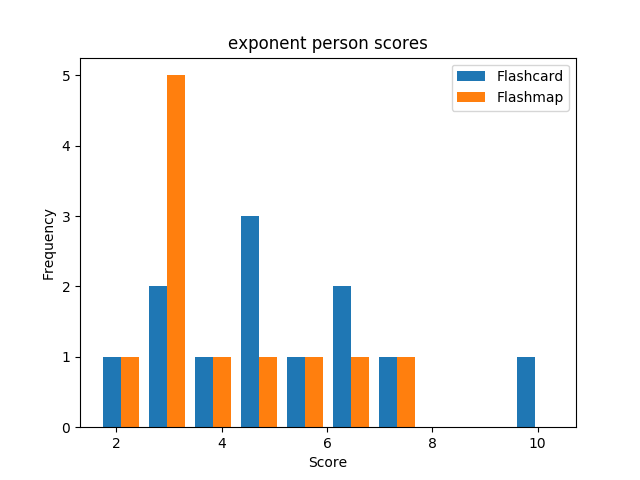
\includegraphics[width=.7\textwidth]{img/exponent_abil.png}
    \caption{A comparison of figure~\protect\ref{fig:exponent_fc_abil} and~\protect\ref{fig:exponent_fm_abil}}
    \label{fig:exponent_abil}
\end{figure}

\FloatBarrier
\section{Descriptives of percentage of responses marked as correct}

\begin{longtable}[c]{@{}lrrrrrrrrrr@{}}
\caption{Flashcard condition}
\endfirsthead
\toprule\addlinespace
& N & min & max & mean & variance & skew & kurt & norm-t &
norm-p & $\alpha$
\\\addlinespace
\midrule
\textbf{abs} & 12 & 35 & 86 & 62.33 & 267.67 & -0.30 & -1.07 & 0.993 &
0.6086 & 0.9780
\\\addlinespace
\textbf{rel} & 12 & 0.38 & 0.93 & 0.67 & 0.03 & -0.30 & -1.07 & 0.993 & 0.6086
& 0.9780
\\\addlinespace
\textbf{mean} & 12 & 0 & 0 & 0.86 & 0.00 & -0.19 & -0.82 & 0.242 &
0.8859 & 0.9780
\\\addlinespace
\bottomrule
    \label{tab:score_fc}
\end{longtable}

\begin{figure}
    \centering
    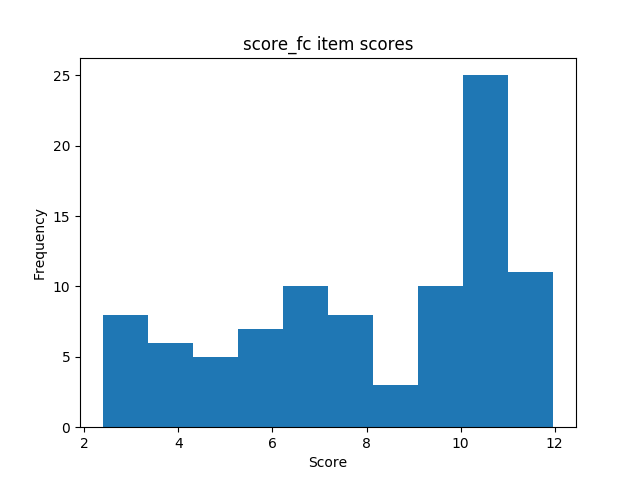
\includegraphics[width=.7\textwidth]{img/score_fc_diff.png}
    \caption{A histogram depicting percentages of correct answers by flashcard users per item}
    \label{fig:score_fc_diff}
\end{figure}
\begin{figure}
    \centering
    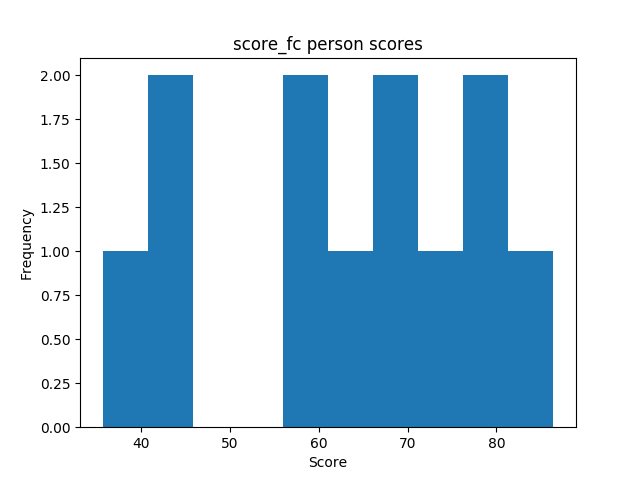
\includegraphics[width=.7\textwidth]{img/score_fc_abil.png}
    \caption{A histogram depicting percentages of correct answers per flashcard user}
    \label{fig:score_fc_abil}
\end{figure}

\begin{longtable}[c]{@{}lrrrrrrrrrr@{}}
\caption{Flashmap condition}
\endfirsthead
\toprule\addlinespace
& N & min & max & mean & variance & skew & kurt & norm-t &
norm-p & $\alpha$
\\\addlinespace
\midrule
\textbf{abs} & 11 & 46 & 185 & 117.55 & 2006.59 & 0.05 & -1.06 & 0.548 &
0.7605 & 0.9928
\\\addlinespace
\textbf{rel} & 11 & 0.23 & 0.93 & 0.59 & 0.05 & 0.05 & -1.06 & 0.548 & 0.7605
& 0.9928
\\\addlinespace
\textbf{mean} & 11 & 0 & 1 & 0.89 & 0.00 & 0.22 & -1.19 & 1.178 & 0.5549
& 0.9928
\\\addlinespace
\bottomrule
    \label{tab:score_fm}
\end{longtable}

\begin{figure}
    \centering
    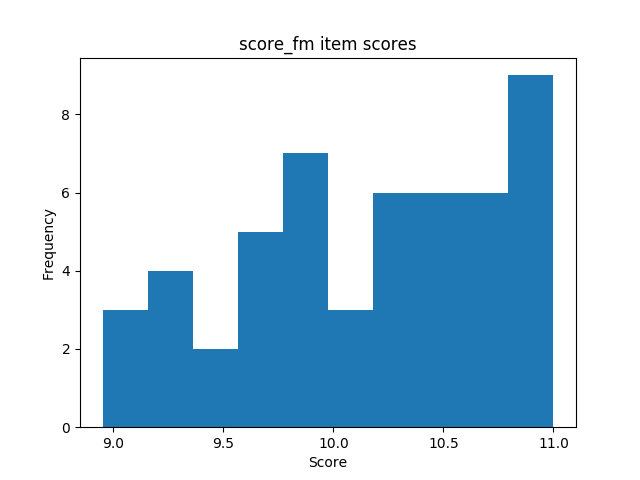
\includegraphics[width=.7\textwidth]{img/score_fm_diff.png}
    \caption{A histogram depicting percentages of correct answers by flashmap users per item}
    \label{fig:score_fm_diff}
\end{figure}
\begin{figure}
    \centering
    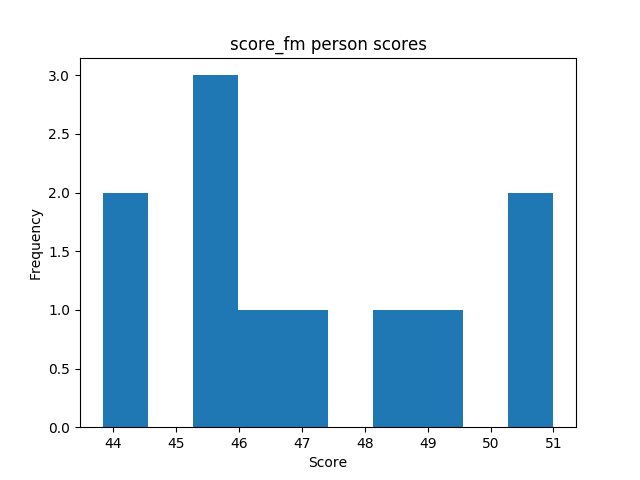
\includegraphics[width=.7\textwidth]{img/score_fm_abil.png}
    \caption{A histogram depicting percentages of correct answers per flashmap user}
    \label{fig:score_fm_abil}
\end{figure}

\begin{longtable}[c]{@{}lrrrrrrrrrr@{}}
\caption{Combined conditions}
\endfirsthead
\toprule\addlinespace
& N & min & max & mean & variance & skew & kurt & norm-t &
norm-p & $\alpha$
\\\addlinespace
\midrule
\textbf{abs} & 23 & 35 & 185 & 88.74 & 1841.51 & 0.93 & -0.13 & 4.256 & 0.1191 & 0.9910
\\\addlinespace
\textbf{mean} & 23 & 0 & 1 & 0.87 & 0.00 & 0.07 & -0.67 & 0.272 & 0.8728
& 0.9910
\\\addlinespace
\bottomrule
    \label{tab:score_gen}
\end{longtable}

\begin{figure}
    \centering
    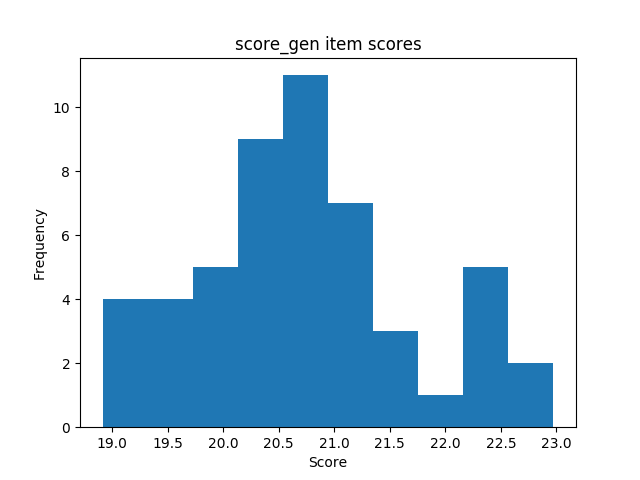
\includegraphics[width=.7\textwidth]{img/score_gen_diff.png}
    \caption{A histogram depicting percentages of correct answers per item}
    \label{fig:score_gen_diff}
\end{figure}
\begin{figure}
    \centering
    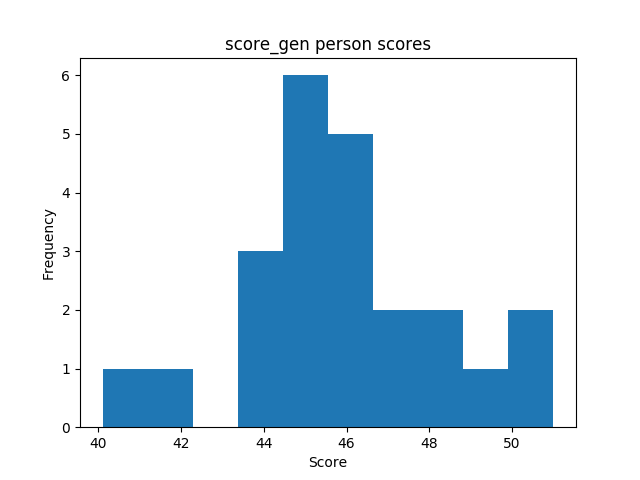
\includegraphics[width=.7\textwidth]{img/score_gen_abil.png}
    \caption{A histogram depicting percentages of correct answers per user}
    \label{fig:score_gen_abil}
\end{figure}

\section{Comparisons of the percentage of responses marked as correct}

\begin{longtable}[c]{@{}lrrrr@{}}
\toprule\addlinespace
& \textbf{MW k} & \textbf{MW p} &
\textbf{t-test k} & \textbf{t-test p}
\\\addlinespace
\midrule
\textbf{abs} & -16.597 & 0.0000 & -15.857 & 0.0000
\\\addlinespace
\textbf{rel} & -16.421 & 0.0000 & -15.689 & 0.0000
\\\addlinespace
\textbf{mean} & -12.448 & 0.0000 & -11.895 & 0.0000
\\\addlinespace
\bottomrule
    \label{tab:score_comp}
\end{longtable}

\begin{figure}
    \centering
    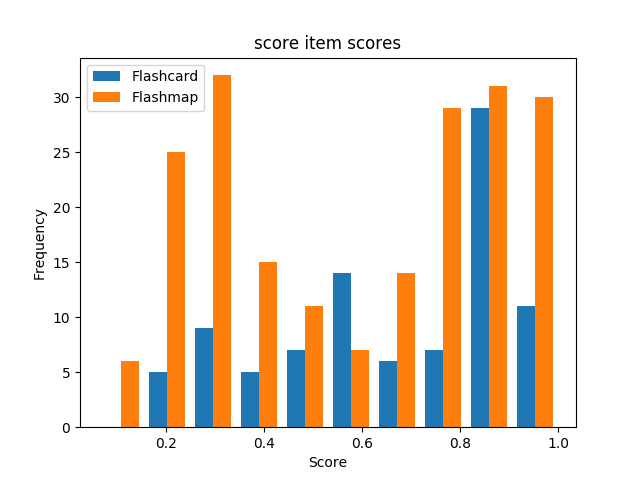
\includegraphics[width=.7\textwidth]{img/score_diff.png}
    \caption{A comparison of figure~\protect\ref{fig:score_fc_diff} and~\protect\ref{fig:score_fm_diff}}
    \label{fig:score_diff}
\end{figure}
\begin{figure}
    \centering
    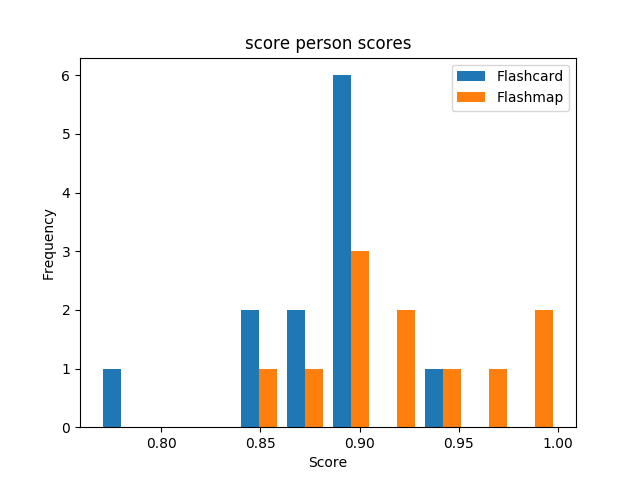
\includegraphics[width=.7\textwidth]{img/score_abil.png}
    \caption{A comparison of figure~\protect\ref{fig:score_fc_abil} and~\protect\ref{fig:score_fm_abil}}
    \label{fig:score_abil}
\end{figure}

\FloatBarrier
\section{Descriptives of the amount of time spent on the application}

\begin{longtable}[c]{@{}lrrrrrrrrrr@{}}
\caption{Flashcard condition}
\endfirsthead
\toprule\addlinespace
& N & min & max & mean & variance & skew & kurt & norm-t &
norm-p & $\alpha$
\\\addlinespace
\midrule
\textbf{abs} & 12 & 1697 & 19721 & 12374.41 & 26140529.78 & -0.61 &
-0.33 & 1.445 & 0.4855 & 0.9239
\\\addlinespace
\textbf{rel} & 12 & 18 & 212 & 133.06 & 3022.38 & -0.61 & -0.33 & 1.445
& 0.4855 & 0.9239
\\\addlinespace
\textbf{mean} & 12 & 35 & 249 & 169.77 & 3881.30 & -1.00 & 0.11 & 4.064
& 0.1311 & 0.9239
\\\addlinespace
\bottomrule
    \label{tab:time_fc}
\end{longtable}

\begin{figure}
    \centering
    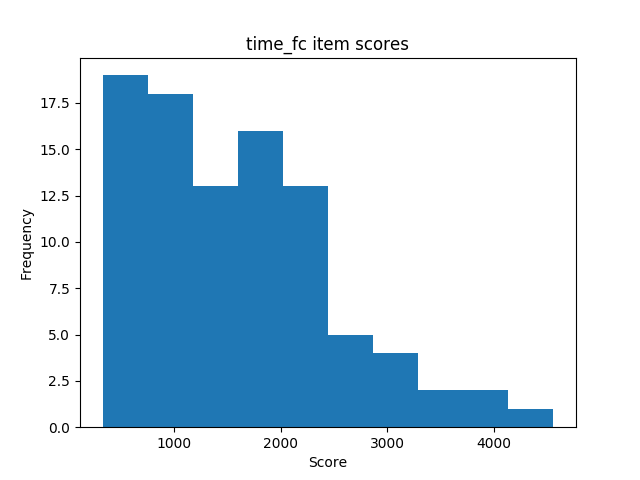
\includegraphics[width=.7\textwidth]{img/time_fc_diff.png}
    \caption{A histogram depicting the time spent in seconds per item by flashcard users} 
    \label{fig:time_fc_diff}
\end{figure}
\begin{figure}
    \centering
    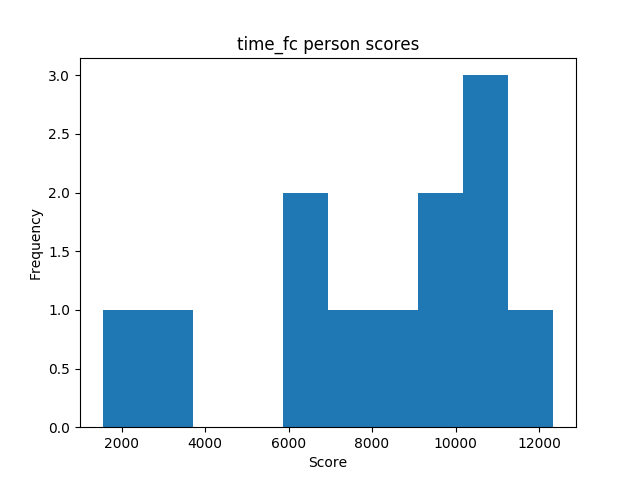
\includegraphics[width=.7\textwidth]{img/time_fc_abil.png}
    \caption{A histogram depicting the time spent in seconds per flashcard user}
    \label{fig:time_fc_abil}
\end{figure}

\begin{longtable}[c]{@{}lrrrrrrrrrr@{}}
\caption{Flashmap condition}
\endfirsthead
\toprule\addlinespace
& N & min & max & mean & variance & skew & kurt & norm-t &
norm-p & $\alpha$
\\\addlinespace
\midrule
\textbf{abs} & 11 & 2612 & 26869 & 14121.58 & 51451085.83 & 0.65 & -0.07
& 1.907 & 0.3854 & 0.9501
\\\addlinespace
\textbf{rel} & 11 & 13 & 135 & 70.96 & 1299.24 & 0.65 & -0.07 & 1.907 &
0.3854 & 0.9501
\\\addlinespace
\textbf{mean} & 11 & 19 & 224 & 117.30 & 3303.44 & 0.24 & -0.34 & 0.380
& 0.8271 & 0.9501
\\\addlinespace
\bottomrule
    \label{tab:time_fm}
\end{longtable}

\begin{figure}
    \centering
    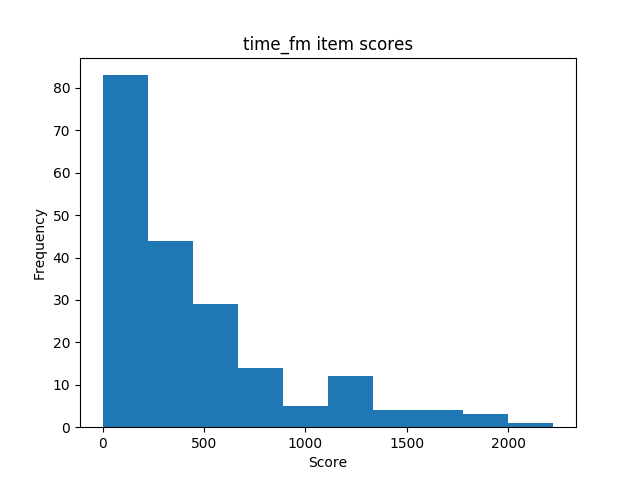
\includegraphics[width=.7\textwidth]{img/time_fm_diff.png}
    \caption{A histogram depicting the time spent in seconds per item by flashmap users} 
    \label{fig:time_fm_diff}
\end{figure}
\begin{figure}
    \centering
    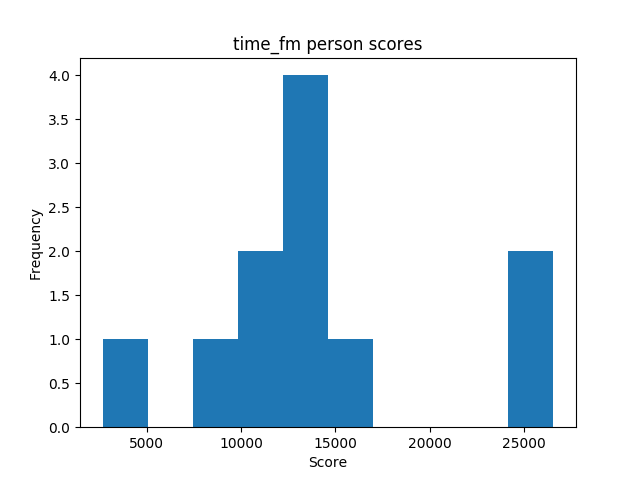
\includegraphics[width=.7\textwidth]{img/time_fm_abil.png}
    \caption{A histogram depicting the time spent in seconds per flashmap user}
    \label{fig:time_fm_abil}
\end{figure}

\begin{longtable}[c]{@{}lrrrrrrrrrr@{}}
\caption{Combined conditions}
\endfirsthead
\toprule\addlinespace
& N & min & max & mean & variance & skew & kurt & norm-t &
norm-p & $\alpha$
\\\addlinespace
\midrule
\textbf{abs} & 23 & 1697 & 26869 & 13210.01 & 37253452.58 & 0.43 & 0.55
& 2.350 & 0.3088 & 0.9281
\\\addlinespace
\textbf{mean} & 23 & 19 & 249 & 144.67 & 4160.26 & -0.29 & -0.93 & 1.630
& 0.4427 & 0.9281
\\\addlinespace
\bottomrule
    \label{tab:time_gen}
\end{longtable}

\begin{figure}
    \centering
    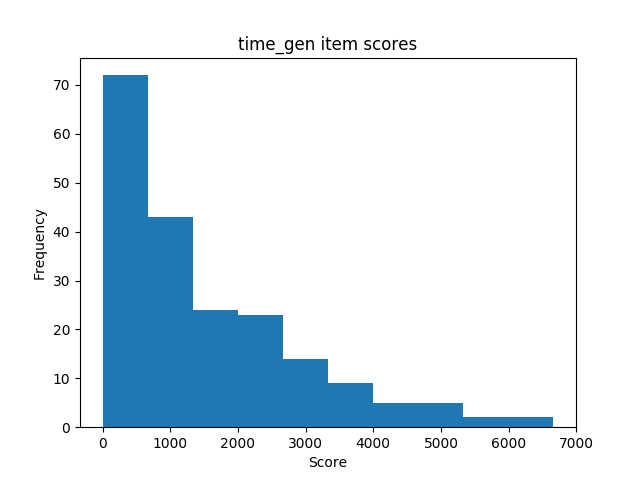
\includegraphics[width=.7\textwidth]{img/time_gen_diff.png}
    \caption{A histogram depicting the time spent in seconds per item} 
    \label{fig:time_gen_diff}
\end{figure}
\begin{figure}
    \centering
    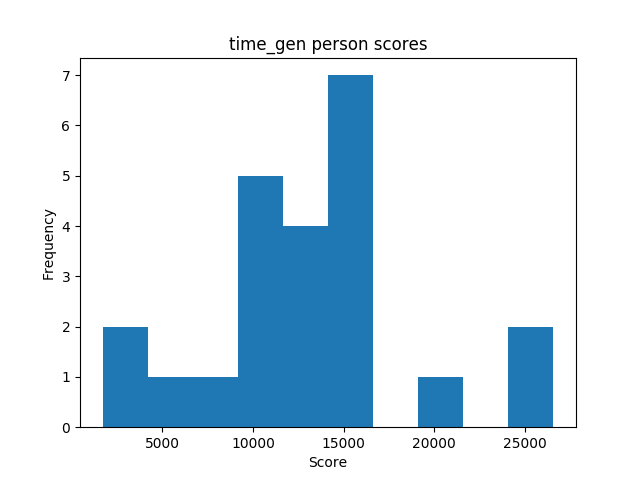
\includegraphics[width=.7\textwidth]{img/time_gen_abil.png}
    \caption{A histogram depicting the time spent in seconds per user}
    \label{fig:time_gen_abil}
\end{figure}

\section{Comparisons of the amount of time spent on the application}

\begin{longtable}[c]{@{}lrrrr@{}}
\toprule\addlinespace
& \textbf{MW k} & \textbf{MW p} &
\textbf{t-test k} & \textbf{t-test p}
\\\addlinespace
\midrule
\textbf{abs} & 7.522 & 0.0000 & 7.869 & 0.0000
\\\addlinespace
\textbf{rel} & 7.787 & 0.0000 & 8.148 & 0.0000
\\\addlinespace
\textbf{mean} & 8.720 & 0.0000 & 9.126 & 0.0000
\\\addlinespace
\bottomrule
    \label{tab:time_comp}
\end{longtable}

\begin{figure}
    \centering
    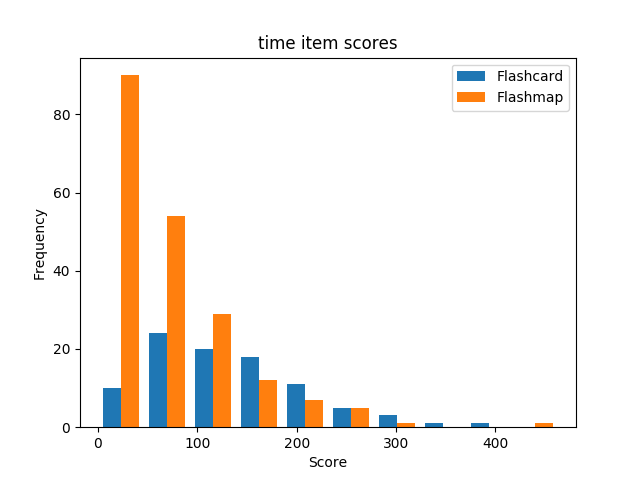
\includegraphics[width=.7\textwidth]{img/time_diff.png}
    \caption{A comparison of figure~\protect\ref{fig:time_fc_diff} and~\protect\ref{fig:time_fm_diff}}
    \label{fig:time_diff}
\end{figure}
\begin{figure}
    \centering
    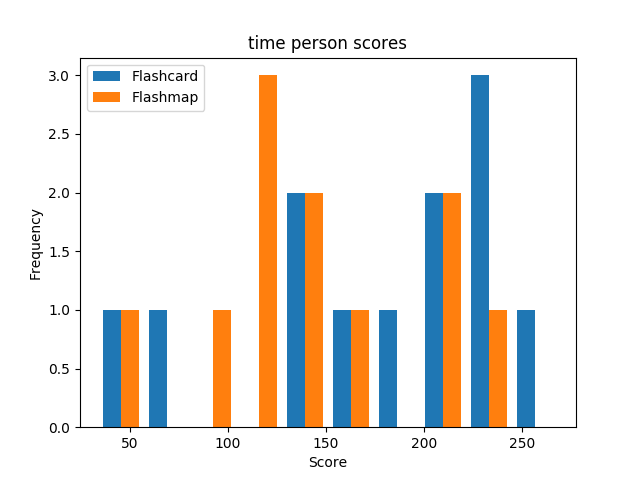
\includegraphics[width=.7\textwidth]{img/time_abil.png}
    \caption{A comparison of figure~\protect\ref{fig:time_fc_abil} and~\protect\ref{fig:time_fm_abil}}
    \label{fig:time_abil}
\end{figure}
